\section{Dinaturality, extranaturality, co/wedges.}\label{section:due}
\epigraph{Los idealistas arguyen que las salas hexagonales son una forma necesaria del espacio absoluto o, por lo menos, de nuestra intuición del espacio.}{J.L\@. Borges, \emph{La biblioteca de Babel}.}
This first section starts with a simple example. Let $\Sets$ denote the category of sets and functions, considered with its natural cartesian closed structure: this means we have a bijection of sets
\[
\Sets(A\times B,C)\cong \Sets(A, C^B)
\]
where $C^B$ is the set of all functions $B\to C$, and that this bijection is natural in each argument. The adjunction $\firstblank\times B\dashv (\firstblank)^B$ has a counit, which is a natural transformation
\[
\epsilon_{X,(B)} \colon X^B\times B\to X
\]
where the codomain can be considered ``mutely depending on the variable $B$''.

The collection of functions $\{\epsilon_X\colon  X^B\times B\to X\}$ is natural in the classical sense in the variable $X$; as for the variable $B$, the most we can say is that for each $f\in \Sets(B,B')$ the following square is commutative:
\[
\vcenter{\xymatrix{
X^{B'}\times B \ar[r]^{X^f\times B}\ar[d]_{X^{B'}\times f}& X^B\times B \ar[d]^{\epsilon}\\
X^{B'}\times B' \ar[r]_{\epsilon}& X
}}
\]
This relation however doesn't remind naturality so much. We address the reader also to Exercise \textbf{2}  at the end of \cite[\textbf{IV.7}]{McL} and our Exercise \textbf{1}.\refbf{ex1:counit.is.cowedge}: it is easy to show that this commutativity is what remains when the naturality in $B$ of the adjunction $\Sets(A\times B,C)\cong \Sets(A, C^B)$ is imposed.% implies a more complicated dependence on the variable $B$.

Fortunately, a suitable generalization of naturality (a ``super-naturality'' condition), encoding the above commutativity, is available to describe this and other similar phenomena putting them in the same common framework.% A notion of super-naturality adapted to describe co/ends as suitable universal objects comes in two flavours: one of them is \emph{di}naturality, which we now introduce.
\begin{definition}[Dinatural Transformation]
Given two functors $P,Q\colon \C^\opp\times \C\to \D$ a \emph{dinatural transformation}, depicted as an arrow $\alpha\colon P\xto{..} Q$, consists of a family of arrows $\{\alpha_c\colon P(c,c)\to Q(c,c)\}_{c\in\C}$ such that for any $f\colon c\to c'$ the following hexagonal diagram commutes
\[
\vcenter{\xymatrix{
P(c',c) \ar[r]^{P(f,c)}\ar[d]_{P(c',f)} & P(c,c) \ar[r]^{\alpha_c} & Q(c,c) \ar[d]^{Q(c,f)}\\
P(c',c') \ar[r]_{\alpha_{c'}} & Q(c',c') \ar[r]_{Q(f, c')} & Q(c,c')
}}
\]
\end{definition}
\begin{definition}[Wedge for a functor]
Let $P\colon \C^\opp\times\C\to\D$; a \emph{wedge} for $P$ is a dinatural transformation $\Delta_d\xto{..}P$ from the constant functor on the object $d\in\D$ (often denoted simply by $d\colon \C^\opp\times\C\to\D$), defined sending $(c,c')\mapsto d$,  $(f,f')\mapsto \id_d$.
\end{definition}
\begin{definition}[End of a functor]
The \emph{end} of a functor $F\colon\C^\opp\times\C\to \D$ consists of a universal wedge $\eend(F) \xto{..}F$; the constant $\eend(F) \in \D$ is itself termed, by abuse, the end of the functor.

Spelled out explicitly, the universality requirement means that for any other wedge $\beta\colon d\xto{..}F$ the diagram
\[
\vcenter{\xymatrix{
d \ar@{.>}[dr]^h \ar@/^1pc/[drr]^{\beta_c}\ar@/_1pc/[ddr]_{\beta_{c'}} & \\
& \eend(F) \ar[r]^{\omega_c}\ar[d]_{\omega_{c'}} & F(c,c) \ar[d]^{F(1,f)} & c \ar[d]^f\\
&F(c',c') \ar[r]_{F(f,1)}& F(c,c') & c'
}}
\]
commutes for a unique arrow $h\colon d\to \eend(F)$, for any arrow $f\colon c\to c'$.
\end{definition}
\begin{remark}
As it is well-known, uniqueness requirements imply functoriality: given a natural transformation $\eta\colon F\Rightarrow F'$ there is an induced arrow $\eend(\eta)\colon \eend(F)\to \eend(F')$ between their ends, as depicted in the diagram
\[
\vcenter{\xymatrix@R=5mm@C=5mm{
&\eend(F') \ar[rr]\ar[dd]|\hole&& F'(c',c')\ar[dd]\\
\eend(F) \ar@{.>}[ur]\ar[rr]\ar[dd]&& F(c',c')\ar[dd]\ar[ur]\\
&F'(c,c) \ar[rr]|(.49)\hole&& F'(c,c')\\
F(c,c) \ar[ur]\ar[rr]&& F(c,c')\ar[ur]
}}
\]
This implies that taking sending a functor $T$ into its end $\eend(T)$ is a (covariant) functor $\D^{\C^\opp\times \C}\to \D$. The case of a coend is dually analogous: filling the details is an easy dualization exercise.
\end{remark}
%\subsection{Extranaturality}
A slightly less general, but better behaved notion of super-naturality (we say ``better behaved'' since it admits a \emph{graphical calculus} translating commutativity\hyp{}checking into checking that certain string diagrams can be deformed one into the other), that allows again to define co/wedges, is available: this notion is called \emph{extra-naturality} and it was introduced in \cite{eilenberg1966generalization}.
\begin{definition}[Extranatural transformation]\label{extranatural}
Let $P,Q$ be functors
\begin{gather*}
P\colon \A\times \cate{B}^\opp\times\cate{B}\to \D\\
Q\colon \A\times \C^\opp\times\C \to \D.
\end{gather*}
An \emph{extranatural transformation} $\alpha\colon P\xto{..}Q$ consist of  a collection of arrows 
\[
\big\{\alpha_{abc}\colon P(a,b,b) \longrightarrow Q(a, c,c)\big\}
\]
indexed by triples of object in $\A\times\B\times\C$ such that the following hexagonal diagram commutes for every $f\colon a\to a'$, $g\colon b\to b'$, $h\colon c\to c'$, all taken in their suitable domains:
\[
\vcenter{\xymatrix@C=1.6cm{
P(a,b',b) \ar[r]^{P(f,b',g)}\ar[d]_{P(a,g,b)} & P(a', b', b') \ar[r]^{\alpha_{a'b'c}} & Q(a', c,c) \ar[d]^{Q(a', c,h)}\\
P(a,b,b) \ar[r]_{\alpha_{abc'}} & Q(a, c', c') \ar[r]_{Q(f,h,c')} & Q(a', c, c');
}}
\]
\end{definition}
Notice how commutative hexagon can be equivalently described as the juxtaposition of three distinguished commutative squares, depicted in \cite{eilenberg1966generalization}: the three can be obtained letting respectively $f$ and $h$, $f$ and $g$, or $g$ and $h$ be identities in the former diagram, which collapses to
\begin{gather}
\label{extrana}
\xymatrix{
P(a, b,b) \ar[r]^{P(f,b,b)}\ar[d]_{\alpha_{abc}}&\ar[d]^{\alpha_{a'bc}} P(a', b,b) \\
Q(a,c,c) \ar[r]_{Q(f,c,c)}& Q(a', c,c)
}\quad 
\xymatrix{
P(a,b',b) \ar[r]^{P(a,b',g)}\ar[d]_{P(a,g,b)}&\ar[d]^{\alpha_{ab'c}} P(a, b', b') \\
P(a,b,b) \ar[r]_{\alpha_{abc}}& Q(a, c,c)
}\quad 
\xymatrix{
P(a,b,b) \ar[r]^{\alpha_{abc}}\ar[d]_{\alpha_{abc'}}&\ar[d]^{Q(a,c,h)} Q(a, c,c) \\
Q(a, c', c') \ar[r]_{Q(a,h,c')}& Q(a, c, c')
}
\end{gather}
\begin{remark}
We can again define co/wedges in this setting: if $\cate{B}=\C$ and in $F(a,b,b)\to G(a,c,c)$ the functor $F$ is constant in $d\in\C$, $G(a,c,c)=\bar G(c,c)$ is mute in $a$, we get a wedge condition for $d\xto{..}G$; dually we obtain a cowedge condition for $F(b,b)\to G(a,b,b)\equiv d'$ for all $a,b,c$. It's worth to notice that a extranatural transformation contains strictly more information than a dinatural, since in \adef\ref{extranatural} we are given arrows $F(b,b) \xto{\alpha_{bb'}} G(b',b')$ that form a cowedge in $b$ for each $b'$, and a wedge in $b'$ for all $b\in\B$.
\end{remark}
Both notions give rise to the same notion of co/end, defined as a universal co/wedge for a bifunctor $F\colon \C^\opp\times\C\to \D$. The main reason we should prefer extranaturality, as was pointed out to the author in a (semi)private conversation with T\@. Trimble, is that
\begin{quote}
\small 
%For the purposes of describing end/coend calculus, I wouldn't emphasize dinatural transformations so much as I would extranatural transformations. 
Most dinatural transformations that arise in the wild can be analyzed in terms of extranatural (extraordinary natural, in the old lingo) transformations. [\dots]

[Co/wedges can be regarded as particular examples of two slightly different, but related (\aprop \refbf{extraisdi}) constructions:] first, they are special examples of dinatural transformations. Second, they are special cases of an extranatural (\emph{extraordinary natural}) transformation, which generally is a family of maps $F(a, a, b) \to G(b, c, c)$ which combines naturality in the argument $b$ with a cowedge condition on $a$ and a wedge condition on~$c$.
\end{quote}
We now briefly describe the promised graphical calculus for extranatural transformations: it depicts the components $\alpha_{abc}$, and arrows $f\colon a\to a'$, $g\colon b\to b'$, $h\colon c\to c'$, as planar diagrams like
\begin{center}
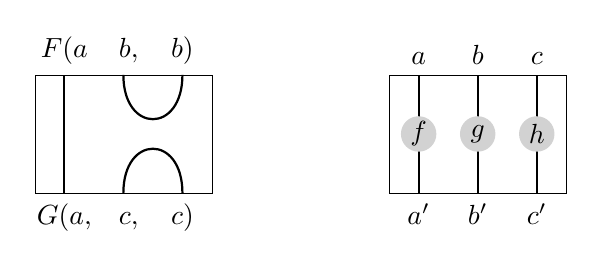
\begin{tikzpicture}[scale=1.5]
% standard block
\begin{scope}[thick]
\draw[ultra thin] (0.25,0) -- (1.75,0) -- (1.75,1) -- (0.25,1) -- cycle;
\draw (.5,0) node[below] {$G(a,$} -- (.5,1) node[above] {$F(a$} ;
\draw (1,0) node[below] {$\phantom{(}c,$} .. controls (1,.5) and (1.5,.5) .. (1.5,0) node[below] {$c)$};
\draw (1,1) node[above] {$\phantom{(}b,$} .. controls  (1,.5) and (1.5,.5) .. (1.5,1) node[above] {$b)$};
\end{scope}

% I parametri sono: 
% - posizione all'interno della striscia (yshift)
% - posizione laterale (xshift)
% - presenza di un nodo e posizione del nodo.
\begin{scope}[thick, xshift=3cm]
\draw[ultra thin] (0.25,0) -- (1.75,0) -- (1.75,1) -- (0.25,1) -- cycle;
\draw (.5,0) node[below] {$a'$} -- (.5,1) node[above] {$a$};
\draw[xshift=.5cm] (.5,0)node[below] {$b'$}  -- (.5,1) node[above] {$b$};
\draw[xshift=1cm] (.5,0) node[below] {$c'$}-- (.5,1) node[above] {$c$};
\filldraw[lightgray!70] (.5,.5) circle (4pt) node[black] {$f$};
\filldraw[lightgray!70] (1,.5) circle (4pt) node[black] {$g$};
\filldraw[lightgray!70] (1.5,.5) circle (4pt) node[black] {$h$};
\end{scope}
\end{tikzpicture}
\end{center}
where wires are labeled by objects and must be thought oriented from top to bottom. The commutative squares of (\refbf{extrana}) become, in this representation, the following three string diagrams, whose equivalence is graphically obvious (the labels $f,g,h$ can ``slide'' along the wire they live in):
\begin{center}
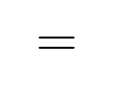
\begin{tikzpicture}[thick, scale=.9]
\standard
\begin{scope}[yshift=-1cm]
\first{f}
\end{scope}
\begin{scope}[xshift=2.5cm]
\first{f}
\end{scope}
\begin{scope}[xshift=2.5cm, yshift=-1cm]
\standard
\end{scope}
\draw (2.25,0) node {\huge $=$};
\end{tikzpicture}
$\quad$
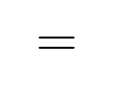
\begin{tikzpicture}[thick, scale=.9]
\second{g}
\begin{scope}[yshift=-1cm]
\standard
\end{scope}
\begin{scope}[xshift=2.5cm]
\third{g}
\end{scope}
\begin{scope}[xshift=2.5cm, yshift=-1cm]
\standard
\end{scope}
\draw (2.25,0) node {\huge $=$};
\end{tikzpicture}
$\quad$
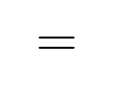
\begin{tikzpicture}[thick, scale=.9]
\standard
\begin{scope}[yshift=-1cm]
\second{h}
\end{scope}
\begin{scope}[xshift=2.5cm]
\standard
\end{scope}
\begin{scope}[xshift=2.5cm, yshift=-1cm]
\third{h}
\end{scope}
\draw (2.25,0) node {\huge $=$};
\end{tikzpicture}
\end{center}
\begin{remark}
The notion of extranatural transformation can be specialized to encompass various other constructions: simple old naturality arises when $F, G$ are both constant in their co/wedge components, like in 
\begin{center}\begin{tikzpicture}[thick, scale=1.4]
\standardbis{black}{dashed,black!40}{dashed,black!40}
\end{tikzpicture}\end{center}
whereas wedge and cowedge conditions arise when either $F,G$ are constant:
\begin{center}\begin{tikzpicture}[thick, scale=1.4]
\standardbis{dashed, black!40}{black}{dashed, black!40}

\begin{scope}[xshift=4cm]
\standardbis{dashed, black!40}{dashed, black!40}{black}
\end{scope}
\end{tikzpicture}\end{center}
All the others mixed situations (a wedge\hyp{}cowedge condition, naturality and a wedge, etc. which lack a specified name) admit a graphical representation of the same sort, and follow similar graphical rules of juxtaposition.
\end{remark}
\begin{proposition}\label{extraisdi}
Extranatural transformations are particular kinds of dinatural transformations.
\end{proposition}
\begin{proof}[Proof (due to T\@.~Trimble)]
Suppose you have functors $F\colon \C^\opp \times \C \times \C \to \D$ and $G\colon \C \times \C \times \C^\opp \to \D$. Now put $\A = \C \times \C^\opp \times \C^\opp$, and form two new functors $F', G': \A^\opp \times \A \to \D$ by taking the composites 
\begin{gather*}
F' =  (\C^\opp \times \C \times \C) \times (\C \times \C^\opp \times \C^\opp) \xto{\text{proj}} \C^\opp \times \C \times \C \xto{F} \D  \\
(x', y', z'; x, y, z) \longmapsto (x', x, y') \stackrel{F}{\mapsto}  F(x', x, y')
\\
{}\\
G' = (\C^\opp \times \C \times \C) \times (\C \times \C^\opp \times \C^\opp)  \xto{\text{proj}'} \C \times \C \times \C^\opp \xto{G} \D\\ 
(x', y', z'; x, y, z)  \mapsto (y', z', z)  \stackrel{G}{\mapsto} G(y', z', z) 
\end{gather*}
Now let's put $a' = (x', y', z')$ and $a = (x, y, z)$, considered as objects in $\A$. An arrow $\phi\colon a' \to a$ in $\A$ thus amounts to a triple of arrows $f\colon x' \to x$, $g\colon y \to y'$, $h\colon z \to z'$ all in $\C$. 

Following the instructions above, we have $F'(a', a) = F(x', x, y')$ and $G(a', a) = G(y', z', z)$. 

Now if we write down a dinaturality hexagon for $\alpha: F' \stackrel{..}{\to} G'$, we get a diagram of shape 
\[
\vcenter{\xymatrix{
F'(a, a') \ar[d]_{F(\phi, 1)}\ar[r]^{F'(1, \phi)} & F'(a, a) \ar[r]^{\alpha_a} & G'(a, a) \ar[d]^{G'(\phi, 1)} \\ 
F'(a', a') \ar[r]_{\alpha_{a'}} & G'(a', a') \ar[r]_{G'(1, \phi)} & G(a', a)
}}\]
which translates to a hexagon of shape 
\[
\vcenter{\xymatrix{
F(x, x', y) \ar[d]_{F(f, 1, g)} \ar[r]^{F(1, f, 1)} & F(x, x, y) \ar[r] & G(y, z, z) \ar[d]^{G(g, h, 1)}\\
F(x', x', y') \ar[r] & G(y', z', z') \ar[r]_{G(1, h, 1)} & G(y', z', z)
}}
\]
where the unlabeled arrows refer to the extranatural transformation. 
\end{proof}
There are, however, dinatural transformations which are not extranatural: an example of such is given in Exercise \refbf{ex1:dinatarentextra}.
\subsection{The integral notation for co/ends}
A suggestive and useful notation alternative to the anonymous one ``$\underline{\text{co}}/\eend(F)$'' is due to N\@.~Yoneda, which in \cite{yoneda} introduces most of the notions we are dealing with, in the setting of $\Ab$\hyp{}enriched functors $\C^\opp\times \C\to \Ab$: the \emph{integral notation} denotes the end of a functor $F\in \D^{\C^\opp\times \C}$ as a ``subscripted\hyp{}integral'' $\int_cF(c,c)$, and the coend $\coend(F)$ as the ``superscripted\hyp{}integral'' $\int^cF(c,c)$.

From now on we will systematically adopt this notation to denote the universal co/wedge $\underline{\text{co}}/\eend(F)$ or, following a well\hyp{}established abuse of notation, the object itself; we also accept slightly more pedantic variants of this, as
\[
\int_{c\in \C}^{/c\in \C}F(c,c), \qquad \int_{c:\C}^{/c:\C}F(c,c).
\]
\begin{remark}
One should be aware that Yoneda reverses this definition since he calls \emph{integrations} our coends, which he denotes as $\int_{c\in\C} F(c,c)$, and \emph{cointegrations} our ends, which he denotes $\int_{c\in\C}^*F(c,c)$. Modern notation complies with the current use of \emph{co-} to denote an initial object.
\end{remark}
\begin{remark}
Properties of co/ends acquire a particularly suggestive flavour when written in this notation:
\begin{enumerate}[label=\oldstylenums{\arabic*})]
\item \textbf{Functoriality} (the \emph{B-rule} for integrals or the \emph{freshman's dream} that the integral of a product is the product of integrals): the unique arrow $\eend(\eta)$ induced by a natural transformation $\eta\colon F\Rightarrow G$ between $F,G\in\D^{ \C^\opp \times \C }$ can be written as $\int\eta\colon \int F\to \int G$, and uniqueness of this induced arrow entails that $\int (\eta\circ\sigma)=\int \eta\circ\int \sigma$.
\item The \textbf{Fubini theorem} for ends, which first appeared as equation (\textbf{4.0.1}) of \cite{yoneda}: given a functor $F\colon \C^\opp\times\C\times \cate{E}^\opp\times \cate E\to \D$, we can form the end $\int_cF(c,c,\firstblank,\secondblank)$ obtaining a functor $\cate{E}^\opp\times \cate E\to \D$ whose end is $\int_e\int_cF(c,c,e,e)\in \D$; we can also form the ends $\int_c\int_e F(c,c,e,e)\in \D$ and $\int_{(c,e)}F(c,c,e,e)$ identifying $\C^\opp\times\C\times \cate{E}^\opp\times \cate E$ with $(\C\times\cate E)^\opp\times (\C\times\cate E)$. \emph{Fubini's theorem} for ends states that there is a canonical isomorphism between the three:
\[
\int_{(c,e)}F(c,c,e,e)\cong 
\int_e\int_cF(c,c,e,e)\cong 
\int_c\int_e F(c,c,e,e)
\]
\end{enumerate}
\end{remark}
\begin{remark}
In some sense, the Fubini rule for coends seems a rather weak analogy allowing to compare integrals and coends; there is no doubt that the following passage (\cite[\textbf{IX.5}]{McL})
\begin{quote}
[\dots] the ``variable of integration'' $c$ [in $\int_c F$] appears twice under the integral sign (once contravariant, once covariant) and is ``bound'' by the integral sign, in that the result no longer depends on $c$ and so is unchanged if $c$ is replaced by any other letter standing for an object of the category $\C$.
\end{quote}
motivates this notation, and yet the analogy itself seems to be too elusive to justify.% In the eye of the author, it seems worthwhile to remember that in view of the characterization for co/ends in terms of co/equalizers given in our subsequent \refbf{endsareeq}, $\int_c\colon \D^{ \C^\opp \times \C }\to \D$ can be thought as an \emph{averaging} operation on a functor, giving the ``fixed points'' of the ``action'' induced by $F(\varphi, c'), F(c,\varphi)$ as $\varphi\colon c\to c'$ runs over $\hom(\C)$.

Although the author prefers to abstain from any further investigation, having no chance to give a valid (or rather, formal) explanation of the integral notation, it is nevertheless impossible to underestimate the power of this convenient shorthand.
\end{remark}
\subsection{Co/ends as co/limits}\label{coends.as.colims}
A general tenet of elementary category theory is that you can always characterize a universal construction as an element of the triad 
\begin{center}
limit - adjoint - representation of functors. 
\end{center}
The formalism of co/ends makes no exception: the scope of the following subsection is to characterize, if it exists, the co/end of a functor $F\colon \C^\opp\times\C\to \D$ as a co/limit over a suitable diagram $\overline F$ (hopefully obtained with a universal construction $F\mapsto \overline F$), and finally as the co/equalizer of a single pair of arrows.

First of all notice that given $F\colon \C^\opp\times \C\to \D$ and a wedge $\tau\colon d\xto{..} F$, we can build the following commutative diagram
\[
\vcenter{\xymatrix@R=.4cm@C=.4cm{
& F(c,c) \ar[rr]^{F(c, f)} & & F(c,c ')\ar[dd]^{F(c, g)}\\
d\ar[ur]^{\tau_c}\ar@/_1pc/[rrrd]|(.67)\hole_{\tau_{gf}}\ar[rr]^{\tau_{c'}}\ar[dd]_{\tau_{c''}} &&  F(c', c')\ar[dd]\ar[ur]_{F(f, c')} \\
& && F(c, c'')\\
F(c'', c'') \ar[rr]_{F(g, c'')} && F(c', c'')\ar[ur]_{F(f, c'')}
}}
\]
where
$c\xto{f}c'\xto{g}c''$ are two arbitrarily chosen, but fixed, arrows in $\C$. From this commutativity we deduce the following relations:
\begin{align*}
\tau_{gf} &=F(gf,c'')\circ \tau_{c''} = F(c,gf)\circ \tau_c\\
&=F(f,c'')\circ F(g,c'')\circ \tau_{c''}=F(f,c'')\circ \tau_g\\
&=F(c,g)\circ F(c,f)\circ\tau_c = F(c,g)\circ \tau_f.
\end{align*}
where $\tau_f$, $\tau_g$ are the common values $F(f, c')\tau_{c'} = F(c,f)\tau_c$ and $F(c',g)\tau_{c'} = F(g, c'')\tau_{c''}$ respectively, $\tau_{gf}$ is the common value $F(c,g)\tau_f = F(f, c'') \tau_g$. These relations imply that there is a link between co/wedges and co/cones, encoded in the following definition.\footnote{I am indebted to \textsf{G. Mossa} (Università degli studi di Pisa, e chissà per quanto) for having revealed me this argument when I was still unable to manipulate co/ends.} 
\begin{definition}[The twisted arrow category of $\C$]\label{twisted}
For every category $\C$ we define $\tw(\C)$, the category of \emph{twisted arrows} in $\C$ as follows:
\begin{itemize}
\item $\text{Ob}(\tw(\C))=\hom(\C)$ (of course, this is not $\mho$-small if $\C$ was only $\mho^+$-small);
\item Given $f\colon c\to c'$, $g\colon d\to d'$ a morphism $f\to g$ is given by a pair of arrows $(h\colon d\to c,k\colon c'\to d')$, such that the obvious square commutes (asking that the arrow between domains is in reversed order is \emph{not} a mistake).
\end{itemize}
\end{definition}
Endowed with the obvious rules for composition and identity, $\tw(\C)$ is easily seen to be a category, and now we can find a functor
\[
\vcenter{\xymatrix{
\text{Fun}(\C^\opp\times\C,\D)\ar[rr]&&\text{Fun}(\tw(\C),\D)
}}
\]
defined sending $F$ to the functor $\overline F\colon \tw(\C)\to \D\colon f\mapsto F(\text{src}(f),\text{trg}(f))$; it is extremely easy now to check that bifunctoriality for $F$ exactly corresponds to functoriality for $\overline F$, but there is more.
\begin{remark}\label{is.a.colim}
The family $\{\tau_f\}_{f\in\hom(\C)}$ constructed before is a cone for the functor $\overline F$, and conversely any such cone determines a wedge for $F$, given by $\{\tau_c\defequal\tau_{\id_c}\}_{c\in \C}$. Again, a morphism of cones maps to a morphism between the corresponding wedges, and conversely any morphism between wedges induces a morphism between the corresponding cones; these operations are mutually inverse and form an equivalence between the category $\textsc{cn}(\overline F)$ of cones for $\overline F$ and the category $\textsc{wd}(F)$ of wedges for $F$ (see Exercise \textbf{1}.\refbf{wedgecat}).
\end{remark}
Equivalences of categories obviously respect initial/terminal objects, and since co/limits are initial/terminal objects in the category of co/cones, and co/ends are initial/terminal objects in the category of co/wedges, we obtain that\footnote{Notice that the colimit is taken over the category $\tw^\opp(\C)$, the \emph{opposite} of $\tw(\C^\opp)$: an \emph{object} of $\tw^{op}(\C)$ is an arrow $f \colon c'\to c$ in $\C^\opp$, and a \emph{morphism} from $f \colon c\to c'$ to $g \colon d \to d'$ is a commutative square $(u,v)$ such that $vgu = f$.}
\[
\int_c F\cong \varprojlim_{\tw(\C)} \overline F; \qquad 
\int^c F\cong \varinjlim_{\tw(\C^\opp)^\opp} \overline F
\]
\begin{remark}
There is another (slightly \emph{ad hoc} and cumbersome, in the humble opinion of the author) characterization of co/ends as co/limits, given by \cite[Prop\@. \textbf{IX.5.1}]{McL}, which relies upon the \emph{subdivision (associative) plot} (see \cite[Def\@. \textbf{2}, \textbf{3}]{Salvo}) $(\wp \C)^\S$ of $\C$, whose
\begin{itemize}
\item objects are the set $\ob(\C)\sqcup\hom(\C)$, in such a way that there exists a ``marked'' object $c^\S$ for each $c\in\C$, and another marked object $f^\S$ for each $f\in\hom(\C)$ (so that $c^\S$ and $\id_c^\S$ are \emph{different} objects of $\C^\S$);
\item arrows are the set of all symbols $\text{src}(f)^\S\to f^\S$, or $\text{trg}(f)^\S\to f^\S$, as $f$ runs over $\hom(\C)$;
\item composition law is the empty function.
\end{itemize}
The \emph{subdivision category} $\C^\S$ is obtained from $(\wp \C)^\S$ formally adding identities and giving to the resulting category the trivial composition law (composition is defined only if one of the arrows is the identity). The discussion before \cite[Prop\@. \textbf{IX.5.1}]{McL} now sketches the proof that every functor $F\colon \C^\opp\times \C\to \D$ induces a functor $\overline F\colon\C^\S\to \D$, whose limit (provided it exists) is isomorphic to the end of $F$.
\end{remark}
\begin{remark}\label{endsareeq}
Co/limits in a category exist whenever the category has co/products and equalizers. So we would expect a  characterization of co/ends in terms of these simpler pieces; such a characterization exists, and it turns out to be extremely useful in explicit computations (see for example our Remark \refbf{theyre.adjoints} and the argument therein). 

In fact it is rather easy to extract from the bare universal property that
\[
\vcenter{\xymatrix{
\int_c F(c,c) \cong \text{eq}\left( \displaystyle \prod_{c\in\C} F(c,c) \ar@<3pt>[r]^(.6){F^*}\ar@<-3pt>[r]_(.6){F_*}\right.& \left.\displaystyle \prod_{\varphi\colon c\to c'} F(c,c')\right)
}}
\]
must be an equalizer, where the product over ${\varphi\colon c\to c'}$ can be expressed as a double product (over the objects $c,c'\in \C$, and over the arrows $\varphi$ between these two fixed objects), and the arrows $F^*, F_*$ are easily obtained from the arrows whose $(\varphi, c,c')$\hyp{}components are (respectively) $F(\varphi, c')$ and $F(c, \varphi)$.
\end{remark}
It is useful to stress that this characterization is compatible with the description of a co/limit as a co/equalizer, when $F$ is mute in one variable. From this we deduce a different argument showing that the co/end of a mute functor coincides with its co/limit.
\begin{definition}
There is an obvious definition of \emph{preservation} of co/ends from their description as co/limits, which reduces to the preservation of the particular kind of co/limit involved in the definition of $\eend(F)$ and $\coend(F)$.
\end{definition}
This remark entails easily that 
\begin{theorem}\label{coconti}
Every co/continuous functor $F\colon \D\to\cate{E}$ preserves every co/end that exists in $\D$, namely if $T\colon \C^\opp\times\C\to \D$ has a co/end $\int_c^{/c} T(c,c)$, then 
\[
F\Big(\textstyle \int_c^{/c} T(c,c) \Big) \cong \int_c^{/c} FT(c,c)
\]
in the obvious meaning that the two objects are canonically isomorphic having the same universal property.
\end{theorem}
As a particular example of this, we have
\begin{corollary}[The $\hom$ functor commutes with integrals]\label{commuhom}
Continuity of the $\hom$ bifunctor $\C(\firstblank,\secondblank)\colon \C^\opp\times\C\to\cate{Sets}$ gives its co/end preservation properties: for every $c\in \C$ we have the canonical isomorphisms
\begin{gather*}
\C\Big( \int^x F(x,x),c \Big)  \cong \int_x \C(F(x,x),c)\\
\C\Big(c, \int_x F(x,x)\Big)\cong \int_x\C(c,F(x,x))
\end{gather*}
\end{corollary}
\begin{remark}
The power of this remark can't be overestimated: co/continuity of the $\hom$ functor is a fundamental \emph{kata} of coend\hyp{}fu. Basically \emph{every} example in the rest of the paper involves a computation carried on using this co/end preservation property, plus the fully faithfulness of the Yoneda embedding.
\end{remark}
\subsection{Natural transformations as ends}
A basic example exploiting the whole machinery introduced so far is the proof that the set of natural transformations between two functors $F,G\colon \C\to \D$ can be characterized as an end:
\begin{theorem}\label{naturalu}
Given functors $F,G\colon \C\to \D$ between small categories we have the canonical isomorphism of sets
\[
\Nat(F,G)\cong \int_c \D(Fc,Gc).
\]
\end{theorem}
\begin{proof}
Giving a wedge $\tau_c\colon Y\to \D(Fc,Gc)$ consists in giving a function $y\mapsto \tau_{c,y}\colon Fc\to Gc$, which is natural in $c\in \C$ (this is simply a rephrasing of the wedge condition):
\[
G(f)\circ \tau_{c,y} = \tau_{c',y}\circ F(f)
\]
for any $f\colon c\to c'$; this means that there exists a unique way to close the diagram
\[
\vcenter{\xymatrix{
Y \ar[r]^{\tau_c}\ar@{.>}@/_1pc/[dr]_h & \D(Fc,Gc)  \\
 & \Nat(F,G) \ar[u]
}}
\]
with a function sending $y\mapsto \tau_{\firstblank,y}\in \prod_{c\in\C} \D(Fc,Gc)$, and where $\Nat(F,G)\to\D(Fc,Gc)$ is the wedge sending a natural transformation to its $c$\hyp{}component; the diagram commutes for a single $h\colon Y\to \Nat(F,G)$, and this is precisely the desired universal property for $\Nat(F,G)$ to be $\int_c\D(Fc,Gc)$.
\end{proof}
\begin{remark}
A suggestive way to express naturality as a ``closure'' condition is given in \cite[\textbf{4.1.1}]{yoneda}, where for an $\Ab$\hyp{}enriched functor $F\colon \C^\opp\times \C\to \Ab$ between suitably complete $\Ab$\hyp{}categories, one can prove that $\Nat(F,G)=\ker\delta$, for a suitable map $\delta$ defined among $\Ab(Fx, Gx)\oplus \Ab(Fy, Gy)$ and $\Ab(Fy, Gy)$.
\end{remark}
After this, we can embark in more sophisticated and pervasive examples. In particular, the following section is the gist of the paper, demonstrating the power of co/end calculus to prove highly technical and involved results by means of abstract\hyp{}nonsense only.
\begin{exerciseset}
\begin{exercisepoints}
\item \label{ex1:counit.is.cowedge} Show that for each $f\in \Sets(B,B')$ the following square is commutative:
\[
\vcenter{\xymatrix{
X^{B'}\times B \ar[r]^{X^f\times B}\ar[d]_{X^{B'}\times f}& X^B\times B \ar[d]^{\epsilon}\\
X^{B'}\times B' \ar[r]_{\epsilon}& X
}}
\]
\item \label{ex1:dinatarenat} A dinatural transformation serves to define natural transformations between functors having the same co/domain but different variance; try to do this.
\item \label{ex1:donotcomp} Show with an example that dinatural transformations $\alpha\colon P\xto{..} Q, \beta\colon Q\xto{..} R$ cannot be composed in general. Nevertheless, there exists a ``composition'' of a dinatural $\alpha\colon P\xto{..}Q$ with a natural $\eta\colon P'\to P$ which is again dinatural $P'\xto{..}Q$, as well as a composition $P\xto{..}Q\to Q'$ (hint: the appropriate diagram results as the pasting of a dinaturality hexagon and two naturality squares).
\item \label{ex1:defcoend} Coends are obtained by a suitable dualization. State the definition of a \emph{cowedge} for a functor $F\colon \C^\opp\times\C\to\D$; a \emph{coend} for $F$ consists of a universal cowedge $\coend(F)$ for $P$. Prove functoriality for coends. Show that coends are ends in the dual category: the coend of $F$ is the end of $F^\opp\colon \C\times\C^\opp\cong \C^\opp\times\C \to \D^\opp$.
\item \label{wedgecat} Define a category $\textsc{wd}(F)$ having objects the wedges for $F\colon \C^\opp\times\C\to\D$ and show that the end of $F$ is the terminal object of $\textsc{wd}(F)$; dualize to coends (initial objects of a category $\textsc{cwd}(F)$ of cowedges).
\item \label{ex1:compoextra} Show that extranatural transformations compose accordingly to these rules:
	\begin{itemize}
	\item (stalactites) Let $F, G$ be functors of the form $\C^\opp \times \C \to \D$. If $\alpha_{x, y}\colon F(x, y) \to G(x,y)$ is natural in $x, y$ and $\beta_x\colon G(x, x) \to H$ is extranatural in $x$ (for some object $H$ of $D$), then 
	\[\beta_x \circ \alpha_{x, x}: F(x, x) \to H\]
	is extranatural in $x$.
	\item (stalagmites) Let $G, H$ be functors of the form $\C^\opp \times \C \to \D$. If $\alpha_x\colon F \to G(x, x)$ is extranatural in $x$ (for some object $F$ of $D$) and $\beta_{x, y}\colon G(x, y) \to H(x, y)$ is natural in $x, y$, then 
	\[
	\beta_{x, x} \circ \alpha_x: F \to H(x, x)
	\]
	is extranatural in $x$. 
	\item (yanking) Let $F, H$ be functors of the form $\C \to \D$, and let $G\colon \C \times \C^\opp \times \C \to \D$ be a functor. If $\alpha_{x, y}\colon F(y) \to G(x, x, y)$ is natural in $y$ and extranatural in $x$, and if $\beta_{x, y}\colon G(x, y, y) \to H(x)$ is natural in $x$ and extranatural in $y$, then 
	\[\beta_{x, x}\circ \alpha_{x, x}\colon F(x) \to H(x)\]
	is natural in $x$. 
	\end{itemize}
Express these laws as equalities between suitable string diagrams (explaining also the genesis of the names ``stalactite'' and ``stalagmite'').
\item \label{ex1:dinatarentextra} (Suggested by {\sf B. Ruggiero} and {\sf L. Perticone}, Università di Roma ``La Sapienza'') This exercise provides a counterexample to the converse implication of \aprop\refbf{extraisdi}, showing that dinaturality is strictly more general than extranaturality. Let $\Delta[1]=\{ 0 \to 1 \}$ be the ``walking arrow'' category, and $S,T \colon \Delta[1]^\opp\times \Delta[1] \to \Set$ the functors respectively defined by
\[
\vcenter{
	\xymatrix{
	\{1\}\ar@{}[dr]|S\ar[r]^{c_1}\ar[d] & \{1,2\}\ar[d]^\sigma & (0,0)\ar[r]\ar[d] & (0,1)\ar[d]& \{1\} \ar[r]\ar[d]\ar@{}[dr]|T & \{1\}\ar[d]^{c_2}\\
	\{1\} \ar[r]_{c_2} & \{1,2\} 	 		  & (1,0) \ar[r] & (1,1) &		  \{1\} \ar[r]_{c_2} & \{1,2\}
	}
}
\]
where $c_i$ chooses element $i\in\{1,2\}$, and $\sigma$ permutes the two elements. Show that there exists a dinatural transformation $T \xto{..} S$, whose components are identities, which is not extranatural when in \adef\refbf{extranatural} we choose $\A=*$ and $\B =\C^\opp$.
\item \label{ex1:provefubini} Prove the Fubini theorem for ends embarking in a long exercise in universality; prove that if $F\colon \C^\opp\times\C\to \D$ is \emph{mute} in one of the two variables (\ie $F(c', c)=\bar F(c)$ or $\hat F(c')$ for each $c,c'\in\C$ and suitable functors $\bar F\colon \C\to\D$ or $\hat F\colon \C^\opp\to \D$), then the co/end of $F$ is canonically isomorphic to its co/limit. This gives an alternative proof of a similar \emph{Fubini rule for co/limits}: given a functor $F\colon I\times J\to \D$ we have
\[\textstyle 
\varinjlim_I \varinjlim_J F\cong \varinjlim_J \varinjlim_I F\cong \varinjlim_{I\times J}F
\]
(and similarly for limits).
\item \label{ex1:vector-of-coends} Introduced to vector analysis in basic calculus courses, students learn that if $(X, \Omega, \mu)$ is a measure space, the integral of a vector function $\vec F \colon X \to \mathbb{R}^n$ such that each $F_i = \pi_i \circ F\colon X\to \mathbb R$ is measurable and has finite integral, is the vector whose entries are $\Big(\int_X F_1 d\mu, \cdots, \int_X F_n d\mu \Big)$. 

Prove that category theory possesses a similar formula, \ie that if $F\colon \C^\opp\times \C \to \A_1\times \cdots \times \A_n$ is a functor towards a product of categories, such that 
for $1\le i\le n$
\begin{itemize}
\item each $\A_i$ has both an initial and a terminal object, respectively denoted $\varnothing$ and $1$;
\item each co/end $\int_c^{/c} \pi_i\circ F$ exists 
\end{itemize}
then the ``vector'' of all these co/ends, as an object $\Big( \int_c^{/c} F_1 , \dots, \int_c^{/c} F_n) \in \A_1\times\cdots \times \A_n$, is the (base of a universal co/wedge forming the) co/end of $F$. 
\item \label{ex1:theresafinal} The categories $\tw(\C)$ and $\C^\S$ are linked by a \emph{final} (see \cite[\textbf{2.11.1}]{Bor1}) functor $K\colon \C^{\S}\to \tw(\C)$; this motivates the fact that the colimit is the same when indexed by one of the two. Define $K$ and show that is is final, \ie that for every object in $\tw(\C)$ the comma category $(\varphi\downarrow K)$ is nonempty and connected (see \cite[Remark \textbf{7.2.10}, Example \textbf{8.3.9}]{riehl2014categorical}).
\item \label{ispull} Show that the end of a functor $T\colon \Delta[1]^\opp\times \Delta[1]\to \Sets$ is the pullback of the morphisms $T(0,0)\xto{T(0,d_0)} T(0,1)\xot{T(d_0,1)}T(1,1)$, i.e\@. 
\[
	\vcenter{\xymatrix{
     \int_{i\in\Delta[1]} T(i,i) \ar[r]\ar[d] & T(0,0)\ar[d]\\
     T(1,1) \ar[r] & T(0,1)
	}}
\]
is a pullback in $\Sets$ (of course there's nothing special about sets here!).
\item \label{ex1:forgroups} Let $G$ be a topological group, and $\text{Sub}(G)$ the partially ordered (with respect to inclusion) set of its subgroups; let $X$ be a $G$-space, \ie a topological space with a continuous action $G\times X \to X$.

We can define two functors $\text{Sub}(G) \to \Top$, sending $(H\le G) \mapsto G/H$ (this is a covariant functor, and $G/H$ has the induced quotient topology) and $(H\le G)\mapsto X^H$ (the subset of $H$-fixed points for the action; this is a contravariant functor).
\begin{enumerate}
\item Compute the coend 
\[
\int^{H\le G} X^G \times G/H
\] 
in $\Top$ if $G = \Z/2$ has the discrete topology;
\item Give a general rule for $\int^{H\le G} X^G \times G/H$ when $H$ is cyclic with $n$ elements;
\item Let instead $\text{Orb}(G)$ be the \emph{orbit category} of subgroups of $G$, whose objects are subgroups but $\hom(H,K)$ contains $G$-\emph{equivariant} maps $G/H \to G/K$. Let again $X^{\firstblank}$ and $G/\firstblank$ define the same functors, now with different action on arrows. Prove that $\int^{H\in\text{Orb}(G)} X^H \times G/H \cong X$ (\emph{Elmendorf reconstruction}, \cite{Elmendorf1983}).
\item Let $E|F$ be a field extension, and $\{H \subseteq \text{Gal}(E|F)\}$ the partially ordered set of subgroups of the Galois group of the extension. Compute (in the category of \emph{rings})
\[
\int^{H} E^H \times \text{Gal}(H|F)
\]
\end{enumerate}
\item \label{ex1:iscoeq} Dualize the above construction, to obtain a similar characterization for the coend $\int^c F(c,c)$, characterized as the coequalizer of a similar pair $(F^*, F_*)$.
\item \label{ex1:jointlypreserve} Show that the $\hom$ functors $\C(\firstblank,y)$ \emph{jointly preserve} ends (see \cite{McL} for a precise definition of joint preservation); the rough idea is that whenever f$\C(W,y)$ is the end of $\C(F(c,c),y)$ for each $y$, naturally in $y\in\C$, then $W$ is canonically isomorphic to $\int^c F(c,c)$.
\item Define the map $\delta$ above, and show that $\ker\delta\cong \int_y \Ab(Fy, Gy)$ in the above notation; dualize to express a coend as a suitable coequalizer.
\item \label{ex1:niftynat} Prove again Theorem \refbf{naturalu}, using the characterization of $\int_c\D(Fc,Gc)$ as an equalizer: the subset of $\prod_{c\in\C} \D(Fc,Gc)$ you will have to consider is precisely the subset of natural transformations $\{\tau_c\colon Fc\to Gc\mid Gf\circ \tau_c = \tau_{c'}\circ Ff,\;\forall f\colon c\to c'\}$.
This yields the evocative formula
\[
\textsf{Nat}(1_\C, 1_\C) = \textsf{End}(1_\C) \cong \int_c \C(c,c).
\]
Is it possible to give an explicit meaning to the dual construction $\int^c \C(c,c)$ (start with simple examples: $\C$ discrete, $\C$ a finite group, $\C$ a finite groupoid\dots)? Compare also Example \refbf{dualvecspace}.
\item \label{ex1:coendofid} What is the co/end of the identity functor $1_{\C^\opp\times \C}\colon \C^\opp\times \C\to \C^\opp\times \C$? Use the bare definition; use the characterization of co/ends as co/limits; feel free to invoke Exercise~\refbf{ex1:vector-of-coends}. 
\item A preliminary definition for this exercise is the following: a set of objects $S\subset\C$ \emph{finitely generates} a category $\C$ if for each object $X\in\C$ and each arrow $f : s\to c$ from $s\in S$ there is a factorization
\[
s \xrightarrow{g} \coprod_{i=1}^n s_i\xrightarrow{h_c} c
\]
where $h_c$ is an epimorphism and $\{s_1, \dots, s_n\}\subset S$ ($n$ depends on $c$ and $f$).

Suppose $T\colon \C^\opp\times \C\to \Sets$ is a functor, finitely continuous in both variables, and $\C$ is finitely generated by $S$. Then, considering $S$ as a full subcategory $\mathbf{S}\subseteq \C$, and calling $T' := T|_{\mathbf S}\colon \mathbf{S}^\opp\times\mathbf{S} \to \Sets$, we have an isomorphism
\[
\int^{c\in \mathbf{S}} T'(c,c) \cong \int^{c\in \C} T(c,c)
\] 
induced by a canonical arrow $\int^{c\in \mathbf{S}} T'(c,c) \to \int^{c\in \C} T(c,c)$.
\item \label{ex1:acriterion} Let $F\dashv U\colon \C\leftrightarrows \D$ be an adjunction, and $G \colon \D^\opp\times \C\to \E$ a functor; then there is an isomorphism
\[
\int^c G(Fc,c) \cong \int^d G(d,Ud).
\]
Show that a converse of this result is true: if the above isomorphism is true for any $G$ and natural therein, then there is an adjunction $F\dashv U$.
\item Disprove the ``infinite Fubini rule'', \ie the following statement: it is possible to freely group and reorder a $\kappa$-transfinite sequence of integrals for a functor $T \colon \prod_{i < \kappa} \C_i \times \C_i^\opp \to \D$, in such a way that this co/limit of integral suitably ``converges'' to $\int_{\prod C_i} T(c_i, c_i)$.
\end{exercisepoints}
\end{exerciseset}
